\section{Linearization}

\subsection{Find equilibrium point}

The assignment states that the fix point has six of parameters set to zero: $$x=y=z=\phi=\theta=\psi=0$$

If the system is filled out with these parameters a much simpler set of equations is obtained:

\begin{eqnarray}
\dot{x}=v_x \\
\label{eq:simplified state equations start}
\dot{y}=v_y \\
\dot{z}=v_z \\
\dot{v_x}=-\frac{k \ d}{m}v_x \\
\dot{v_y}=-\frac{k \ d}{m}v_y \\
\dot{v_z}=-\frac{k \ d}{m}v_z -g + \frac{K \ C_m}{m}(v_1^2+v_2^2+v_4^2+v_4^2)\\
\dot{\phi}=w_x \\
\dot{\theta}=w_y \\
\dot{\psi}=w_z \\
\dot{w_x}=\frac{L \cdot k \cdot C_m}{I_{xx}}(v_1^2 - v_3^2) - \frac{I_{yy}-I_{zz}}{I_{xx}} w_y  w_z \\
\dot{w_y}=\frac{L \cdot k \cdot C_m}{I_{xx}}(v_2^2 - v_4^2) - \frac{I_{zz}-I_{xx}}{I_{yy}} w_y  w_z\\
\dot{w_z}=\frac{b \cdot C_m}{I_{yy}}(v_1^2-v_2^2+v_3^2-v_4^2) - \frac{I_{xx}-I_{yy}}{I_{zz}}w_y  w_z
\label{eq:simplified state equations stop}
\end{eqnarray}

Its very clear from equations~\ref{eq:simplified state equations start} - \ref{eq:simplified state equations stop} that $v_x,v_y,x_z,w_x,w_y$ and $w_z$ have to be set to zero to get an equilibrium point.  The set of equations \ref{eq:simplified state equations start} - \ref{eq:simplified state equations stop} can now be simplified further: 

\begin{eqnarray}
\dot{v_z}= -g + \frac{K \ C_m}{m}(v_1^2+v_2^2+v_4^2+v_4^2) =0\\
\dot{w_x}=\frac{L \cdot k \cdot C_m}{I_{xx}}(v_1^2 - v_3^2) =0 \\
\dot{w_y}=\frac{L \cdot k \cdot C_m}{I_{xx}}(v_2^2 - v_4^2) =0\\
\dot{w_z}=\frac{b \cdot C_m}{I_{yy}}(v_1^2-v_2^2+v_3^2-v_4^2) =0
\end{eqnarray}

The only remaining undetermined parameter is $v_i$ some of the constant can be left out to create an over simpler set of equations: 

\begin{eqnarray}
g =  \frac{K \ C_m}{m}(v_1^2+v_2^2+v_4^2+v_4^2)\\
v_1^2 - v_3^2 =0 \\
v_2^2 - v_4^2 =0\\
v_1^2-v_2^2+v_3^2-v_4^2 =0
\end{eqnarray}

This implies that:

\begin{eqnarray}
v_1^2 = v_3^2 \\
v_2^2 = v_4^2 \\
\end{eqnarray}

and so:

\begin{equation}
v_1^2=v_2^2=v_3^2=v_4^2
\label{eq:all motors need to run at the same speed}
\end{equation}

Equation~\ref{eq:all motors need to run at the same speed} implies that all the motors need to turn at the same speed, which means that the quad copter will hoover. The speed at which these motors need to rotate depends on the gravity which is the last equation $$g =  \frac{K \ C_m}{m}(v_1^2+v_2^2+v_4^2+v_4^2) \\$$ $$v_1^2+v_2^2+v_3^2+v_4^2=u_1+u_2+u_3+u_4=\frac{m \cdot g}{K \cdot C_m}$$ As all the voltages are exactly the same this becomes: $$\frac{m \cdot g}{K \cdot C_m \cdot 4}=   v_i^2 = u_i $$ with $i=1...4$ 

\subsection{Define linear model}

The lineare model is of the form $$\triangle \dot{x}=A\triangle x + B\triangle u $$ $$ \triangle y=C\triangle x$$

The matrix is the Jacobian related to x and matrix B is the Jacobian related to u both evaluated in the equilibrium point.

$$x=[x \ y \ z \ v_x \ v_y \ v_z \ \phi \ \theta \ \psi \ w_x \ w_y \ w_z]  $$
$$x_{equilibrium} = [0\ 0\ 0\ 0\ 0\ 0\ 0\ 0\ 0\ 0\ 0\ 0]$$

$$
u_{equilibrium} =
 [\frac{m \cdot g}{K \cdot C_m \cdot 4} \frac{m \cdot g}{K \cdot C_m \cdot 4} \frac{m \cdot g}{K \cdot C_m \cdot 4} \frac{m \cdot g}{K \cdot C_m \cdot 4}] 
$$

$$
A(x_{equilibrium}) =
\begin{bmatrix}
0 & 0 & 0 & 1 & 0 & 0 & 0 & 0 & 0 & 0 & 0 & 0 \\
0 & 0 & 0 & 0 & 1 & 0 & 0 & 0 & 0 & 0 & 0 & 0 \\
0 & 0 & 0 & 0 & 0 & 1 & 0 & 0 & 0 & 0 & 0 & 0 \\

0 & 0 & 0 & -\frac{k_d}{m} & 0 & 0 & 0 & g & 0 & 0 & 0 & 0 \\
0 & 0 & 0 & 0 & -\frac{k_d}{m} & 0 & -g & 0 & 0 & 0 & 0 & 0 \\
0 & 0 & 0 & 0 & 0 & -\frac{k_d}{m} & 0 & 0 & 0 & 0 & 0 & 0 \\

0 & 0 & 0 & 0 & 0 & 0 & 0 & 0 & 0 & 1 & 0 & 0 \\
0 & 0 & 0 & 0 & 0 & 0 & 0 & 0 & 0 & 0 & 1 & 0 \\
0 & 0 & 0 & 0 & 0 & 0 & 0 & 0 & 0 & 0 & 0 & 1 \\

0 & 0 & 0 & 0 & 0 & 0 & 0 & 0 & 0 & 0 & 0 & 0 \\
0 & 0 & 0 & 0 & 0 & 0 & 0 & 0 & 0 & 0 & 0 & 0 \\
0 & 0 & 0 & 0 & 0 & 0 & 0 & 0 & 0 & 0 & 0 & 0
\end{bmatrix}
$$
$$
=
\begin{bmatrix}
	0 & 0 & 0 & 1 & 0 & 0 & 0 & 0 & 0 & 0 & 0 & 0 \\
	0 & 0 & 0 & 0 & 1 & 0 & 0 & 0 & 0 & 0 & 0 & 0 \\
	0 & 0 & 0 & 0 & 0 & 1 & 0 & 0 & 0 & 0 & 0 & 0 \\
	
	0 & 0 & 0 & -0.5 & 0 & 0 & 0 & 9.81 & 0 & 0 & 0 & 0 \\
	0 & 0 & 0 & 0 & -0.5 & 0 & -9.81 & 0 & 0 & 0 & 0 & 0 \\
	0 & 0 & 0 & 0 & 0 & -0.5 & 0 & 0 & 0 & 0 & 0 & 0 \\
	
	0 & 0 & 0 & 0 & 0 & 0 & 0 & 0 & 0 & 1 & 0 & 0 \\
	0 & 0 & 0 & 0 & 0 & 0 & 0 & 0 & 0 & 0 & 1 & 0 \\
	0 & 0 & 0 & 0 & 0 & 0 & 0 & 0 & 0 & 0 & 0 & 1 \\
	
	0 & 0 & 0 & 0 & 0 & 0 & 0 & 0 & 0 & 0 & 0 & 0 \\
	0 & 0 & 0 & 0 & 0 & 0 & 0 & 0 & 0 & 0 & 0 & 0 \\
	0 & 0 & 0 & 0 & 0 & 0 & 0 & 0 & 0 & 0 & 0 & 0
\end{bmatrix}
$$



$$
u = [u_1 \ u_2 \ u_3 \ u_4] = [v_1^2 \ v_2^2 \ v_3^2 \ v_4^2 ]
$$

$$
B(u_{equilibrium}) = 
\begin{bmatrix}
0 & 0 & 0 & 0 \\ %x
0 & 0 & 0 & 0 \\ %y
0 & 0 & 0 & 0 \\ %z

0 & 0 & 0 & 0 \\ %vx dot
0 & 0 & 0 & 0 \\ %vy dot
\frac{k c_m}{m} & \frac{k c_m}{m} & \frac{k c_m}{m} & \frac{k c_m}{m} \\

0 & 0 & 0 & 0 \\
0 & 0 & 0 & 0 \\
0 & 0 & 0 & 0 \\

\frac{L K c_m }{I_{xx}} & 0 & -\frac{L K c_m }{I_{xx}} & 0 \\
0 & \frac{L K c_m }{I_{yy}} & 0 & -\frac{L K c_m }{I_{yy}} \\
\frac{b c_m }{I_{zz}} & -\frac{b c_m }{I_{zz}} & \frac{b c_m }{I_{zz}} & -\frac{b c_m }{I_{zz}}\\
\end{bmatrix}
= 
\begin{bmatrix}
0 & 0 & 0 & 0 \\ %x
0 & 0 & 0 & 0 \\ %y
0 & 0 & 0 & 0 \\ %z

0 & 0 & 0 & 0 \\ %vx dot
0 & 0 & 0 & 0 \\ %vy dot
0.06 & 0.06 & 0.06 & 0.06 \\

0 & 0 & 0 & 0 \\
0 & 0 & 0 & 0 \\
0 & 0 & 0 & 0 \\

1.5 & 0 & -1.5 & 0 \\
0 & 1.5 & 0 & -1.5 \\
1 & -1 & 1 & -1\\
\end{bmatrix}
$$

The matrix C should be constructed so the outputs are the position and balance: $x \ y \ z   \ \phi \ \theta \ \psi$

$$
C=
\begin{bmatrix}
1 & 0 & 0 & 0 & 0 & 0 & 0 & 0 & 0 & 0 & 0 & 0 \\
0 & 1 & 0 & 0 & 0 & 0 & 0 & 0 & 0 & 0 & 0 & 0 \\
0 & 0 & 1 & 0 & 0 & 0 & 0 & 0 & 0 & 0 & 0 & 0 \\
0 & 0 & 0 & 0 & 0 & 0 & 1 & 0 & 0 & 0 & 0 & 0 \\
0 & 0 & 0 & 0 & 0 & 0 & 0 & 1 & 0 & 0 & 0 & 0 \\
0 & 0 & 0 & 0 & 0 & 0 & 0 & 0 & 1 & 0 & 0 & 0 \\
\end{bmatrix}
D=
\begin{bmatrix}
0 & 0 & 0 & 0\\0 & 0 & 0 & 0\\0 & 0 & 0 & 0\\
0 & 0 & 0 & 0\\0 & 0 & 0 & 0\\0 & 0 & 0 & 0\\
\end{bmatrix}
$$


\subsection{Test Linear model}
The simplest test of the linear model is to apply an step signal to all motors at the same time. This should only affect the z-axis as can be seen on Figure~\ref{fig:test lin model}. As the equilibrium point take is the one with the quad copter hovering on a static location. 
\begin{figure}[H]
	\centering
	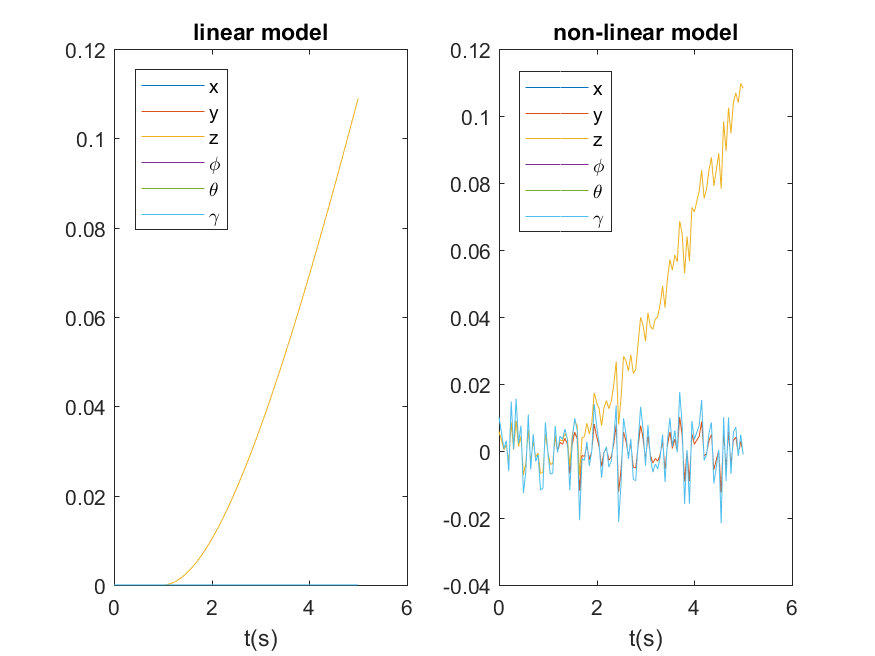
\includegraphics[width=7cm]{./img/lin_approx/step_all.png}
	\caption{step signal to all motors, linear model on the left, non linear on the right}
	\label{fig:test lin model}
\end{figure}